\documentclass{article}
\usepackage{amsmath,amsfonts,amsthm,amssymb}
\usepackage{listings}
\usepackage{xcolor}
\usepackage{setspace}
\usepackage{paralist}
\usepackage{fancyhdr}
\usepackage{lastpage}
\usepackage{extramarks}
\usepackage{chngpage}
\usepackage{color}
% \usepackage{soul,color}
\usepackage{graphicx,float,wrapfig}
\usepackage{mathrsfs}
\usepackage{algorithm}
\usepackage{algorithmic}
\usepackage{tikz}
\definecolor{pblue}{rgb}{0.13,0.13,1}
\definecolor{pgreen}{rgb}{0,0.5,0}
\definecolor{pred}{rgb}{0.9,0,0}
\definecolor{pgrey}{rgb}{0.46,0.45,0.48}
\lstset{language=Java,
  showspaces=false,
  showtabs=false,
  breaklines=true,
  showstringspaces=false,
  breakatwhitespace=false,
  commentstyle=\color{pgreen},
  keywordstyle=\color{pblue},
  stringstyle=\color{pred},
  basicstyle=\ttfamily,
  moredelim=[il][\textcolor{pgrey}]{$$},
  moredelim=[is][\textcolor{pgrey}]{\%\%}{\%\%}
}
\usetikzlibrary{arrows,positioning,automata,shadows,fit,shapes}
% \usepackage{pgffor}
\newcommand{\xd}{\leqslant}
\newcommand{\dd}{\geqslant}
% In case you need to adjust margins:
\topmargin=-0.45in      %
\evensidemargin=0in     %
\oddsidemargin=0in      %
\textwidth=6.5in        %
\textheight=9.0in       %
\headsep=0.25in         %

% Setup the header and footer
\pagestyle{fancy}                                                       %
% \lhead{\StudentName}                                                 %
\chead{\Title}  %
%\rhead{\firstxmark}                                                     %
\lfoot{\lastxmark}                                                      %
\cfoot{}                                                                %
\rfoot{Page\ \thepage\ of\ \protect\pageref{LastPage}}                          %
\renewcommand\headrulewidth{0.4pt}                                      %
\renewcommand\footrulewidth{0.4pt}                                      %

\newcommand{\Proof}{\ \\\textbf{Proof:} }
\newcommand{\Answer}{\ \\\textbf{Answer:} }
\newcommand{\Acknowledgement}[1]{\ \\{\bf Acknowledgement:} #1}

\makeatletter
\newcommand{\rmnum}[1]{\romannumeral #1}
\newcommand{\Rmnum}[1]{\expandafter\@slowromancap\romannumeral #1@}
\makeatother
%%%%%%%%%%%%%%%%%%%%%%%%%%%%%%%%%%%%%%%%%%%%%%%%
%%%%%%%%%%%%%%%%%%%%%%%%%%%%%%%%%%%%%%%%%%%%%%%%
% Make title
\newcommand{\Class}{Operating System}
\newcommand{\ClassInstructor}{Xu Wei}

% Homework Specific Information. Change it to your own
\newcommand{\Title}{Nachos Phase 1 Final Report}
\newcommand{\DueDate}{March 11, 2014}
\title{\textmd{\bf \Class: \Title}\\{\large Instructed by \textit{\ClassInstructor}}\\\normalsize\vspace{0.1in}\small{Due\ on\ \DueDate}}
\date{}

\author{%
  Huang JiaChen 2011012358 \and
  Wu YueXin 2011012xxx \and
  Yang Sheng 2011012359 \and
  Yin HeZheng 2011012343 \and
  Zhou XuRen 2011012xxx}
\newcommand{\StudentClass}{Yao Class}

% \author{\textbf{\StudentName}}
%%%%%%%%%%%%%%%%%%%%%%%%%%%%%%%%%%%%%%%%%%%%%%%%%%%%%%%%%%%%%

  \begin{document}
  \begin{spacing}{1.1}
    \maketitle \thispagestyle{empty}

%%%%%%%%%%%%%%%%%%%%%%%%%%%%%%%%%%%%%%%%%%%%%%%%%%%%%%%%%%%%%%%%%%%%%%%%%%%%%%%%%%%%%%%% Begin edit from here

\theoremstyle{plain} \newtheorem{computational}{Definition}
    \section{Task 1}

    \subsection{Correctness Constraints}
    \begin{enumerate}
      \item[$\bullet$] Caller thread waits (sleep) until callee thread finishes.
      \item[$\bullet$] If callee thread has finishes, \texttt{join()} just returns
	directly.
      \item[$\bullet$] All the threads except caller thread should not be effected.
    \end{enumerate}

    \subsection{Declarations}
    Here, we can see that in order to implement \texttt{join()} method, we need callee
    thread sends a signal to caller thread once callee finished. Therefore, we use
    semaphore to reach this goal.
    \begin{enumerate}
      \item[$\bullet$] \textit{data structures}: \texttt{Semaphore}.
      \item[$\bullet$] \textit{member variable}:
	\begin{enumerate}
	  \item \textbf{private} \texttt{Semaphore KThread::finishSemaphore}, initially 0;
	\end{enumerate}
	indicate whether the thread is finished: \texttt{value} = 0 means unfinished, while
	\texttt{value} = 1 means finished.

    \end{enumerate}

    \subsection{Description}
    because \texttt{KThread::finishSemaphore} is a private
    member variable, we need to modify its value in methord \texttt{finish()}.
    The pseudo code is as follows:
    \begin{algorithm}
      \caption{\texttt{KThread::join()}}
      \begin{algorithmic}[1]
	\STATE /* the given code */
	\STATE finishSemaphore.P();
	\STATE finishSemaphore.V();
      \end{algorithmic}
    \end{algorithm}

    \begin{algorithm}
      \caption{\texttt{KThread::finish()}}
      \begin{algorithmic}[1]
	\STATE /* the given code except sleep() */
	\STATE finishSemaphore.V();
	\STATE sleep(); // this code is the last line in the orginal KThread::finish()
      \end{algorithmic}
    \end{algorithm}

    \subsection{Testing Plan}
    \begin{enumerate}
      \item[] case 1: Only 2 thread, \texttt{thread1} and \texttt{thread2}.
	\texttt{thread1} calls \texttt{thread2.join()} before \texttt{thread2} finishes.
      \item[] case 2: Only 2 thread, \texttt{thread1} and \texttt{thread2}.
	\texttt{thread1} calls \texttt{thread2.join()} after \texttt{thread2} finishes.
      \item[] case 3: Only 3 thread, \texttt{thread1},\texttt{thread2} and
	\texttt{thread3}. \texttt{thread1} calls \texttt{thread2.join()} while
	\texttt{thread2} calls \texttt{thread3.join()}.
    \end{enumerate}
    \section{Task 2}
    \subsection{Implementation}
    \texttt{sleep()}: we can first disable interrupts in order to make a small critical section, in which we only need to put it in a \texttt{ThreadQueue()} and announce it to sleep.

    \texttt{wake()}: it can be realized by taking the first element in the queue out, and call the \texttt{ready()} function.

    \texttt{wakeAll()} can be done by iteratively taking elements out of the queue and call the \texttt{read()} function.

    \subsection{Pseudocode}
    \textit{Variables: }
    \texttt{waitQueue = \color{blue}new ThreadedKernel.scheduler.newThreadQueue(false);} is a \texttt{ThreadQueue} for threads blocked by \texttt{sleep()}.
    \begin{algorithm}
      \caption{ \texttt{void Condition2::sleep()}}
      \begin{algorithmic}
	\STATE Disable interrupts
	\STATE Release \texttt{conditionLock}
	\STATE \texttt{waitQueue.waitForAccess(KThread.currentThread())}
	\STATE	\texttt{KThread.sleep()}
	\STATE Acquire \texttt{conditionLock}
	\STATE Enable interrupts
      \end{algorithmic}
    \end{algorithm}

    \begin{algorithm}
      \caption{ \texttt{void Condition2::wake()}}
      \begin{algorithmic}
	\STATE Disable interrupts
	\IF {\texttt{thread = waitQueue.nextThread() != null}}
	\STATE \texttt{thread.ready()}
	\ENDIF
	\STATE Enable interrupts
      \end{algorithmic}
    \end{algorithm}

    \begin{algorithm}
      \caption{ \texttt{void Condition2::wakeAll()}}
      \begin{algorithmic}
	\STATE Disable interrupts
	\WHILE {\texttt{thread = waitQueue.nextThread() != null}}
	\STATE \texttt{thread.ready()}
	\STATE \texttt{thread = waitQueue.nextThread()}
	\ENDWHILE
	\STATE Enable interrupts
      \end{algorithmic}
    \end{algorithm}

    \subsection{Testing}

    The test is done by running a new static function \texttt{Condition2.selfTest()} which is called in \texttt{ThreadKernel.selfTest()}, and the specific cases are as follows {\color{blue} using a producer-consumer model}:
    \begin{asparaitem}
    \item Case 1: Two threads in which one is sleeper and the other is the waker.
    \item Case 2: Several sleepers with one waker {\color{blue} where the producer can iteratively produce enough number of items}.
    \item Case 3: Several sleepers together with several wakers.
    \end{asparaitem}
    \subsection{Testing Pesudocodes}

    \begin{algorithm}
      \caption{\texttt{Producer::run()}}
      \begin{algorithmic}
        \STATE \texttt{//enqueue items }
        \FOR{\texttt{int i = 0; i < numProducts; i++}}
        \STATE \texttt{lock.acquire(); }
        \STATE \texttt{System.out.println("*** producer " + which + " adds item. "); }
        \STATE \texttt{sharedata.add(which); }
        \STATE \texttt{dataready.wake(); }
        \STATE \texttt{lock.release(); }
        \ENDFOR
      \end{algorithmic}
    \end{algorithm}

    \begin{algorithm}
      \caption{\texttt{Consumer::run()}}
      \begin{algorithmic}
        \STATE \texttt{//dequeue items }
        \STATE \texttt{lock.acquire(); }
        \STATE \texttt{System.out.println("*** consumer " + which + " enters. "); }
        \WHILE{\texttt{sharedata.isEmpty()}}
        \STATE \texttt{System.out.println("*** consumer " + which + " sleeps. "); }
        \STATE \texttt{dataready.sleep(); }
        \ENDWHILE
        \STATE \texttt{System.out.println("*** consumer " + which + " gets " + sharedata.pop() }
        \STATE \texttt{+ "'s item. "); }
        \STATE \texttt{lock.release(); }
      \end{algorithmic}
    \end{algorithm}
    \begin{algorithm}
      \caption{\texttt{ProducerConsumerTest::ProducerConsumerTest(int numProducer, int numConsumer, int productsPerProducer=1)}}
      \begin{algorithmic}
            \STATE \texttt{\color{blue}//Initialize producers and consumers }
            \FOR{\texttt{int i = 0; i < numProducer; i++}}
            \STATE \texttt{producers.push(new Producer(i, productsPerProducer)); }
            \STATE \texttt{order.push(1); }
            \ENDFOR
            \FOR{\texttt{int i = numProducer; i < numProducer + numConsumer; i++}}
            \STATE \texttt{consumers.push(new Consumer(i)); }
            \STATE \texttt{order.push(2); }
            \ENDFOR
            \STATE\texttt{\color{blue} //use random order to execute producers and consumers}
            \STATE \texttt{Collections.shuffle(order); }
            \STATE \texttt{Stack<KThread> joinStack = new Stack<KThread>(); }
            \FOR{\texttt{int i = 0; i < numProducer + numConsumer; i++}}
            \STATE \texttt{int currentNumber = order.pop(); }
            \IF{\texttt{currentNumber == 1}}
            \STATE \texttt{joinStack.push(new KThread(producers.pop())); }
            \STATE \texttt{joinStack.peek().fork(); }
            \ELSIF{(currentNumber == 2)}
              \STATE \texttt{joinStack.push(new KThread(consumers.pop())); }
              \STATE \texttt{joinStack.peek().fork(); }
            \ENDIF
            \ENDFOR
            \WHILE{\texttt{!joinStack.isEmpty()}}
            \STATE \texttt{joinStack.pop().join(); }
            \ENDWHILE
          \end{algorithmic}
        \end{algorithm}

    \begin{algorithm}
      \caption{\texttt{Condition2::selfTest()}}
      \begin{algorithmic}
        \STATE {\color{blue}\texttt{//Case 1: 1 producer, 1 consumer }}
        \STATE \texttt{System.out.println("Case 1:"); }
        \STATE \texttt{new ProducerConsumerTest(1, 1); }
        \STATE {\color{blue}\texttt{ //Case 2: 1 producer, several consumers }}
        \STATE \texttt{System.out.println("Case 2:"); }
        \STATE \texttt{new ProducerConsumerTest(1, 4, 4); }
        \STATE {\color{blue}\texttt{ //Case 3: 3 producer3, 3 consumer3 }}
        \STATE \texttt{System.out.println("Case 3:"); }
        \STATE \texttt{new ProducerConsumerTest(3, 3); }
      \end{algorithmic}
    \end{algorithm}
    \begin{lstlisting}

    \end{lstlisting}

    \section{Task 3}
    \subsection{Implementation}
\begin{asparaitem}
\item Make threads sleep in \texttt{waitUntil(long x)}.

\item In \texttt{timerInterrupt()}, if the current time is larger than a thread's expected waiting time, make a signal.
\end{asparaitem}
\subsection{Code}
\begin{asparaitem}
    \item Class: \texttt{AlarmThread} is a wrapper that associates \texttt{KThread} with wake up time.
    \item Instance: \texttt{queue} is a priority queue \texttt{PriorityQueue<AlarmThread>} that keeps a record of sleeping threads.
    \end{asparaitem}
    \begin{lstlisting}
    public void timerInterrupt() {
    Machine.interrupt().disable();
    //poll threads that have slept for expected
   	while (!queue.isEmpty() &&
			(queue.peek().wakeTime < Machine.timer().getTime())) {
   		queue.poll().thread.ready();
   	}
   	Machine.interrupt().enable();

   	KThread.yield();
    }

    public void waitUntil(long x) {
    Machine.interrupt().disable();
	long wakeTime = Machine.timer().getTime() + x;
    //put threads to sleep
	queue.offer(new AlarmThread(KThread.currentThread(), wakeTime));
	KThread.sleep();
	Machine.interrupt().enable();
    }
    //wrapper class that combines threads with their sleeping time
    private class AlarmThread implements Comparable {
    	AlarmThread(KThread thread, long wakeTime) {
    		this.thread = thread;
    		this.wakeTime = wakeTime;
    	}
		@Override
		public int compareTo(Object o) {
			if (this.wakeTime < ((AlarmThread)o).wakeTime)
				return -1;
			else if (this.wakeTime > ((AlarmThread)o).wakeTime)
				return 1;
			else
				return 0;
		}
		
    	KThread thread;
    	long wakeTime;
    }
    \end{lstlisting}

    \subsection{TESTING}
   The test is done by running a new static function \texttt{Alarm.selfTest()} which is called in \texttt{ThreadKernel.selfTest()}, and the specific cases are as follows {\color{blue} by simply making sleeping threads}:
    \begin{asparaitem}
    \item Case 1: one thread with wait time $0$.
    \item Case 2: one thread with wait time within $500$.
    \item Case 3: one thread with wait time beyond $500$.
    \item Case 4: several threads with arbitrary wait time.
    \end{asparaitem}
  \subsection{Test Pseudocodes}
  \begin{algorithm}
    \caption{\texttt{sleepThread::run()}}
    \begin{algorithmic}
\STATE \texttt{long startTime = Machine.timer().getTime();  }
\STATE \texttt{System.out.println("*** thread " + which + " sleep for " + x + " ticks\ n\ tat time " + startTime); }
\STATE \texttt{ThreadedKernel.alarm.waitUntil(x); }
\STATE \texttt{long currentTime = Machine.timer().getTime(); }
\STATE \texttt{System.out.println("*** thread " + which + " wakes after " }
\STATE \texttt{+ (currentTime - startTime) }
\STATE \texttt{+ " ticks\ n\ tat time " + currentTime); }
    \end{algorithmic}
  \end{algorithm}

  \begin{algorithm}
    \caption{\texttt{Alarm::selfTest()}}
    \begin{algorithmic}
      \STATE {\color{blue}\texttt{//Case 1 }}
      \STATE \texttt{System.out.println("Case 1:"); }
      \STATE \texttt{KThread thread = new KThread(new sleepThread(0, 0)); }
      \STATE \texttt{thread.fork(); }
      \STATE \texttt{thread.join(); }
      \STATE {\color{blue}\texttt{//Case 2 }}
      \STATE \texttt{System.out.println("Case 2:"); }
      \STATE \texttt{thread = new KThread(new sleepThread(1, 100)); }
      \STATE \texttt{thread.fork(); }
      \STATE \texttt{thread.join(); }
      \STATE {\color{blue}\texttt{//Case 3 }}
      \STATE \texttt{System.out.println("Case 3:"); }
      \STATE \texttt{thread = new KThread(new sleepThread(2, 600)); }
      \STATE \texttt{thread.fork(); }
      \STATE \texttt{thread.join(); }
      \STATE {\color{blue}\texttt{//Case 4 }}
      \STATE \texttt{System.out.println("Case 4:"); }
      \STATE \texttt{LinkedList<KThread> threadList = new LinkedList<KThread>();}
      \STATE \texttt{Random rand = new Random(); }
      \FOR{\texttt{int i = 0; i < 5; i++}}
      \STATE \texttt{threadList.add(new KThread(new sleepThread(i + 3, rand.nextInt(400) + 300))); }
      \STATE \texttt{threadList.get(i).fork(); }
      \ENDFOR
      \FOR{\texttt{int i = 0; i < 5; i++}}
      \STATE \texttt{threadList.poll().join(); }
      \ENDFOR
    \end{algorithmic}
  \end{algorithm}

    \section{Task 4}

    \subsection{Correctness Constraints}
    \begin{enumerate}
      \item[$\bullet$] An active speaker should wait until an listener becomes active and
	recieves the word.
      \item[$\bullet$] At any time, there should be at most one active speaker.
      \item[$\bullet$] If there are some waiting speakers but no active speaker,
	some waiting speaker should become active.
      \item[$\bullet$] An active listener should wait until an active speaker becomes
	active and the listener recieves the speaker's word.
      \item[$\bullet$] At any time, there should be at most one active listener.
      \item[$\bullet$] If there are some waiting listeners but no active listener,
	some waiting listener should become active.
      \item[$\bullet$] Once the listener recieves the word, both the speaker and
	the listen should leave.
    \end{enumerate}

    \subsection{Declarations}
    Here we can see that the \texttt{Communicator} is a mutex resource, we need use
    a lock to protect this resource. And we can see that we need to maintain waiting
    speakers and listeners, we can use condition variables to manage them. And we
    can find that active speaker and active listener need to cooperate with other
    threads, we also use condition variables to manage them. Finially, to check whether
    there is active speaker or listener, we use two boolean variables to indicate
    respectively; and we use boolean variable to indicate whether the word is recieved.
    \begin{enumerate}
      \item[$\bullet$] \textit{data structure}: \texttt{Semaphore}, \texttt{Lock}.
      \item[$\bullet$] \textit{member variable}:
	The following variables are all the member variables of \texttt{Communicator},
	all of them are private.
	\begin{enumerate}
	  \item \texttt{Lock lock};
	  \item \texttt{Condition waitingSpeakerQueue}, initially \texttt{lock};
	  \item \texttt{Condition waitingListenerQueue}, initially \texttt{lock};
	  \item \texttt{Condition activeSpeaker}, initially \texttt{lock};
	  \item \texttt{Condition activeListener}, initially \texttt{lock};
	  \item \texttt{boolean noActiveSpeaker}, initially \texttt{true};
	  \item \texttt{boolean noActiveListener}, initially \texttt{true};
	  \item \texttt{boolean recieve}, initially \texttt{false};
	  \item \texttt{int word};
	\end{enumerate}
    \end{enumerate}

    \subsection{Description}

    \begin{algorithm}
      \caption{\texttt{Communicator::speak(w)}}
      \begin{algorithmic}[1]
	\STATE lock.acquire();
	\IF{!noActiveSpeaker}
	\STATE waitingSpeakerQueue.sleep();
	\ENDIF
	\STATE noActiveSpeaker $\leftarrow$ false;
	\STATE word $\leftarrow$ w;
	\IF{noActiveListener or !recieve}
	\STATE activeListener.wake();
	\STATE activeSpeaker.sleep();
	\ENDIF
	\STATE noActiveSpeaker, noActiveListener $\leftarrow$ true;
	\STATE recieve $\leftarrow$ false;
	\STATE waitingSpeakerQueue.wake();
	\STATE waitingListenerQueue.wake();
	\STATE lock.release();
      \end{algorithmic}
    \end{algorithm}

    \begin{algorithm}
      \caption{\texttt{Communicator::listen()}}
      \begin{algorithmic}[1]
	\STATE lock.acquire();
	\IF{!noActiveListener}
	\STATE waitingListenerQueue.sleep();
	\ENDIF
	\STATE noActiveListener $\leftarrow$ false;
	\IF{noActiveSpeaker}
	\STATE activeListener.sleep();
	\ENDIF
	\STATE activeSpeaker.wake();
	\STATE result $\leftarrow$ word;
	\STATE lock.release();
	\RETURN result;
      \end{algorithmic}
    \end{algorithm}

    \subsection{Testing Plan}
    \begin{enumerate}
      \item[] case 1: 1 speaker $\texttt{thread1}$ and 1 delay listener $\texttt{thread2}$,
	and check if $\texttt{thread1}$ wait for $\texttt{thread2}$.
      \item[] case 2: 2 speaker $\texttt{thread1}$,$\texttt{thread2}$ and
	1 listener $\texttt{thread3}$, and check if $\texttt{thread2}$ is blocked.
      \item[] case 3: exchange the position between speaker and listener in case 1 and 2.
      \item[] case 4: 2 speaker and 2 listener and check if they form two pairs.(namely,
	speaker $i$ only speaks to listen $i$, $i=1,2$)
    \end{enumerate}
\section{Task 5}
\subsection{Overview}
Task 5 asks us to implement priority scheduling in Nachos by completing the \texttt{PriorityScheduler} class. Particularly, in choosing which  thread to dequeue, the scheduler always choose a thread of the highest effective priority (choose the one that has been waiting in the queue longest if multiple threads with the same highest priority are waiting).

The most difficulty lies in the function \texttt{Scheduler.getEffectivePriority}. To calculate one thread's effective priority (abbr. EP), we have to maintain a priority queue representing all threads it is getting priority from. Notice that when a thread's EP changes, threads' EP which that thread is waiting on may change as well. So we also need to maintain which thread is it waiting on for each thread.

Specifically, we calculate a thread's prior it  by taking the max of the donor's and the recipient's priority. As for the transitive property of priority donation, we simply call \texttt{Scheduler.getEffectivePriority} recursively.

To speed up the calculation of EP, we create a variable to cache EP in class \texttt{ThreadState}. Thus, we only need to recalculate a thread's effective priority when it is possible for it to change.

\subsection{Correctness Constraints}

\begin{asparaitem}
\item All threads waiting in a queue are sorted by their effective priority\\
\item All threads store a linked list of queues they own and its own effective priority for cache\\
\item The effective priority of a thread is calculated by taking max between its initial priority and the largest effective priority stored in the linked list of queues.\\
\item When a thread is selected from the queue to acquire the resource (\texttt{nextThread}) that thread is removed from the queue and the new thread is told to aquire the queue (\texttt{acquire}) The previous owner of the queue is told it no longer owns this queue, and this queue is removed from its linked list. At the same time, this queue is inserted into the linked list of new owner. The new owner of the queue gets the highest priority in the queue added to its priority cache and its effective priority updated. \\
\item When a thread is added to the waiting queue (\texttt{waitForAccess}), it may have the highest priority of all threads in the queue. The owner of the queue then needs to update its effective priority to be greater than or equal to the new waiting thread.\\
\item When a change occurs to a thread's effective priority, it must reinsert itself into the correct position in the queue and as a result may end up affecting the effective priority of that queue's owner.
\end{asparaitem}

\subsection{Declarations}

We use \texttt{LinkedList<PriorityQueue> waitBy} and \texttt{PriorityQueue waitOn} to store threads waiting us and threads we are waiting separately. The class \texttt{PriorityQueue} is implemented by java.util.PriorityQueue.

\subsection{Descriptions}

The following algorithm describes the implementation of \texttt{getEffectivePriority} in high level.

\begin{algorithm}
  \caption{calculate effective priority}
\begin{algorithmic}[1]
  \STATE Initialize EP and donatorEP as default priority
  \STATE EP $\leftarrow$ priority
\FORALL {wait queues whose resource has been acquired by me}
  \STATE donatorEP $\leftarrow$ largest EP in that wait queue
  \IF {donatorEP $>$ EP}
    \STATE EP $\leftarrow$ donatorEP
  \ENDIF
\ENDFOR
\STATE recursively call calculate effective priority on the thread I am waiting on
\RETURN EP
\end{algorithmic}
\end{algorithm}

To clarify how we manipulate data structure, we illustrate the implementation of function \linebreak \texttt{PriorityQueue.waitForAccess}, \texttt{PriorityQueue.acquire} and \texttt{PriorityQueue.nextThread} (actually, \linebreak \texttt{waitForAccess} and \texttt{acquire} are implemented in class \texttt{ThreadState}).

\begin{algorithm}
  \caption{\texttt{ThreadState.wairForAccess(PriorityQueue waitQueue)}}
\begin{algorithmic}[1]
  \STATE waitQueue.add(this)  \COMMENT{add this thread to waitQueue}
  \STATE this.waitingOn $\leftarrow$ waitQueue  \COMMENT{update waitingOn queue}
  \STATE this.EP $\leftarrow$ calculateEffectivePriority()  \COMMENT{update EP}
\RETURN
\end{algorithmic}
\end{algorithm}

\begin{algorithm}
  \caption{\texttt{ThreadState.acquire(PriorityQueue waitQueue)}}
\begin{algorithmic}[1]
  \STATE waitQueue.owner $\leftarrow$ this
  \STATE this.waitingBy.insert(waitQueue)
  \STATE this.EP $\leftarrow$ calculateEffectivePriority()  \COMMENT{update EP}
\RETURN
\end{algorithmic}
\end{algorithm}

\begin{algorithm}
  \caption{\texttt{nextThread}}
\begin{algorithmic}[1]
  \STATE Initialize chosenThread as null
  \STATE chosenThread $\leftarrow$ pickNextThread()
  \IF {chosenThread != null}
    \STATE remove this queue from current owner's waitingBy list
    \STATE chosenThread.waitingOn $\leftarrow$ null
    \STATE insert this queue into chosenThread's waitingBy list
  \ENDIF
  \STATE this.owner $\leftarrow$ chosenThread
\RETURN chosenThread
\end{algorithmic}
\end{algorithm}

\subsection{Testing Plan}

\section{Task 6}

\subsection{Implemented Strategy}
The strategy implemented is the same as the role-assigning strategy described in our design document. More specifically, we assigned three roles to all threads:
\begin{asparaitem}
  \item \textbf{Rower}: The child who is responsible to row the boat. We denote it by $R$.\\
  \item \textbf{Rider}: The child who is responsible to ride the boat of the rower. We denote it by $D$.\\
  \item Other people who are going to be carried by $R$ and $D$, i.e. passengers. We denote them as $P$.\\
\end{asparaitem}

To carry an adult to Molokai, we used the following subroutine:\\
\begin{asparaitem}
  \item Two children go to Molokai, one rowing the boat and the other riding it.\\
  \item One child rows the boat back to Oahu.\\
  \item The adult rows to Molokai.\\
  \item The child left on Molokai rows the boat back to Oahu.\\
  \item Two children go to Molokai.\\
\end{asparaitem}

Also, to carry a child to Molokai, we used the following subroutine:
\begin{asparaitem}
  \item Two children go to Molokai, one rowing the boat and the other riding it.\\
  \item One child rows the boat back to Oahu.\\
  \item Two children go to Molokai.\\
\end{asparaitem}

The whole carring strategy is just the repeated execution of those two subroutines, and it can be described as follows:

\begin{asparaitem}
  \item We store the total number of adults and children in a global variable. Each time a person is created, the counter increases by one.\\
  \item All the children try to acquire the rower role, and only one of them get it, which is called as $R$.\\
  \item Those who failed to get the rower role try to acquire the rider role, and only one of them get it, which is  called as $D$. All the adults and the children who failed then waits to be carried to Molokai.\\
  \item When $D$ is picked from the children threads, the remaining threads are allowed to go across the sea. There is a global lock which all people except for $R$ and $D$ are waiting to acquire. If one person acquired the lock, he calls $R$ and $D$ to carry him to Molokai via one of the two subrountines, depending on whether it is a child or an adult. Then it decreases the population by 1, release the lock, and returns.\\
  \item At the end no one except $R$ and $D$ is running, and the population counter is 0. Then $R$ and $D$ perform the final rowing to Molokai and returns.
\end{asparaitem}

\subsection{Implementation Code}
\subsubsection{Variables Defined}
\textcolor{green}{In our final implementation, we used almost completely different variables to accomplish the task. The defined variables are used as follows:}
\begin{itemize}
  \item \texttt{int population}: the global population counter, initially 0. When a passenger thread is created, it increments this counter by 1. $R$ and $D$ determined the termination of execution by reading this variable.\\
  \item \texttt{boolean isRowerSet, isRiderSet}: the global indicator indicating whether $R$ and $D$ have been selected. When a child thread is created, it checks and sets these variables and choose to execute $R$, $D$ or $P$ method.\\
  \item \texttt{boolean isAdult}: the indicator indicating whether this $P$ thread being carried is an adult. $R$ checks this variable and determines which protocol to follow.\\
  \item \texttt{Lock move}: Every thread should acquire this lock whenever they are created. This lock takes charge of all threads and makes them follow the protocols.\\
  \item \texttt{Condition mainMove, rowerMove, riderMove, waitingMove, passengerMove}: These conditions are all belong to the lock \texttt{move} and provides queues for different threads to sleep. For example, when $R$ needs to sleep, it will call \texttt{rowerMove.sleep()} to ensure other thread correctly wake it up later on.\\
\end{itemize}

\subsubsection{Codes}
Pseudocodes are presented in the algorithm boxes.\\

\begin{lstlisting}
public static void begin(int adults, int children, BoatGrader b)
{
  bg = b;
  isRowerSet = false;
  isRiderSet = false;
  population = 0;
	
  move = new Lock(); // mutex initializing
  riderMove = new Condition(move);
  rowerMove = new Condition(move);
  passengerMove = new Condition(move);
  waitingMove = new Condition(move);
  mainMove = new Condition(move);
	
  move.acquire();
	
  Runnable child = new Runnable() {
	public void run() {
      ChildItinerary();
    }
  };

  Runnable adult = new Runnable() {
      public void run() {
      AdultItinerary();
    }
  };

  for(int i = 0; i < children; i ++)
  {
    KThread t = new KThread(child);
    t.setName("Child Thread " + i);
    t.fork();
    mainMove.sleep(); // wait for the child initializing
  }
  for(int i = 0; i < adults; i ++)
  {
    KThread t = new KThread(adult);
    t.setName("Adult Thread " + i);
    t.fork();
    mainMove.sleep(); // wait for the adult initializing
  }
  rowerMove.wake(); //wake up rower to start carrying; will be woken up by halting or error
  mainMove.sleep();
}


static void AdultItinerary()
{
  bg.initializeAdult();

  move.acquire();
  population ++;

  mainMove.wake(); // initialization is finished. Start waiting
  waitingMove.sleep();

  // protocol part
  isAdult = true;
  rowerMove.wake();
  passengerMove.sleep();
  bg.AdultRowToMolokai();
  population --;
  rowerMove.wake();
  move.release();

}

static void ChildItinerary()
{
  bg.initializeChild();
  move.acquire();
  population ++;
  if(isRowerSet == false)
  {
    isRowerSet = true;
    Rower();
  }
  else if(isRiderSet == false)
  {
    isRiderSet = true;
    Rider();
  }
  else
  {
    mainMove.wake();
    waitingMove.sleep();

    // protocol part
    isAdult = false;
    rowerMove.wake();
    passengerMove.sleep();
    bg.ChildRideToMolokai();
    population --;
    rowerMove.wake();
  }

  move.release();
}

static void Rower()
{
  mainMove.wake();
  rowerMove.sleep();
  while(population >= 3)
  {
    waitingMove.wake();
    rowerMove.sleep();
    if(isAdult == true) // protocol for adult
    {
      bg.ChildRowToMolokai();
      riderMove.wake();
      rowerMove.sleep();
      passengerMove.wake();
      rowerMove.sleep();
      bg.ChildRowToOahu();
    }
    else // protocol for children
    {
      bg.ChildRowToMolokai();
      passengerMove.wake();
      rowerMove.sleep();
      bg.ChildRowToOahu();
    }
  }
  bg.ChildRowToMolokai();
  riderMove.wake();
}

static void Rider()
{
  mainMove.wake();
  riderMove.sleep();

  while(population >= 3)
  {
    bg.ChildRideToMolokai();
    bg.ChildRowToOahu();
    rowerMove.wake();
    riderMove.sleep();
  }

  bg.ChildRideToMolokai();
  mainMove.wake(); // wake up the main thread to finish
}
\end{lstlisting}

\subsection{Test Taken}
\subsubsection{Correctness Analysis}
To test the correctness of the role-assigning strategy, we created a class \texttt{BoatChecker extends BoatGrader} to take charge of all testing tasks.\\
In our \texttt{selfTest()}, we called \texttt{begin} using a \texttt{BoatChecker} as the final argument. Each time a message is sent to the checker, it examines the following three kinds of errors:\\
\begin{itemize}
  \item State transition error: the state transition is invalid. We will discuss this later on.\\
  \item Population error: all the numbers of children and adults on both side of the sea should be always non-negative. \texttt{bc} will update th epopulation for each call, and if a negative population number is detected, \texttt{bc} will throw out an exception indicating that population error.\\
  \item Halting error: upon halting there should not be anyone on side Oahu. If there are still people waiting for carring when \texttt{begin()} is going to halt, there is a halting error.\\
\end{itemize}
The state of the boat rowing mechanism can be regarded as a DFA below:\\
\begin{center}
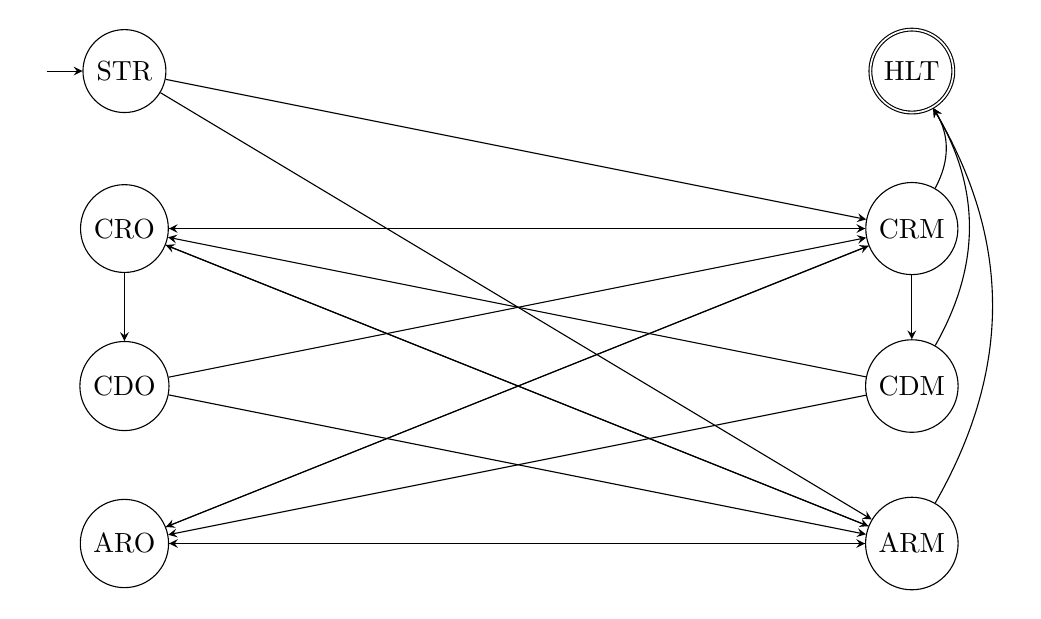
\begin{tikzpicture}[%
	>=stealth,
	node distance = 2cm,
	on grid,
	auto
	]
	\node[initial, initial text = ,state] (str) {STR};
    \node[state] (cro) [below of= str] {CRO};
    \node[state] (cdo) [below of= cro] {CDO};
    \node[state] (aro) [below of= cdo] {ARO};
    \node[state, accepting] (hlt) at (10, 0) {HLT};
    \node[state] (crm) [below of=hlt] {CRM};
    \node[state] (cdm) [below of = crm] {CDM};
    \node[state] (arm) [below of = cdm] {ARM};

    \path[->]
    (str) edge (arm)
    (str) edge (crm)
    (cdo) edge (arm)
    (cdo) edge (crm)
    (cro) edge (arm)
    (cro) edge (crm)
    (aro) edge (arm)
    (aro) edge (crm)
    (crm) edge (cro)
    (crm) edge (aro)
    (cdm) edge (cro)
    (cdm) edge (aro)
    (arm) edge (cro)
    (arm) edge (aro)
    (crm) edge (cdm)
    (cro) edge (cdo)
    (crm) edge [bend right] (hlt)
    (cdm) edge [bend right] (hlt)
    (arm) edge [bend right] (hlt);
\end{tikzpicture}
\end{center}
Here, a state indicates the function it has just implemented: for example, it is permissible to call \texttt{ChildRowToOahu()} (CRO) just after \texttt{ChildRowToMolokai()}, but it is not valid to call \texttt{ChildRideToMolokai()} after \texttt{ChildRowToOahu()}. The DFA is thus responsible for both the position of the boat and the number of person on the boat.\\
Each time a method is called, we check if the transition function is permissible. If so, \texttt{bc} will output an error message.\\
If none of the three kinds of errors occur, the boat rowing scheme will halt normally without any error message. Then \texttt{bc} will output a success message.\\
\subsubsection{Efficiency Analysis}
To carry $a$ adults and $b$ children across the sea, it can be proved that the minimum number of steps is $5a+3b-4$. Each time a method is called, \texttt{bc} will increment a counter \texttt{step}, which is initialized to be 0. When \texttt{begin()} halts normally, \texttt{bc} will output
$$\#\text{Steps taken/ \# Minimum steps}$$
as a measure of efficiency. Analysis related to the clocktick has not been implemented yet.\\
\end{spacing}
To see the \texttt{BoatChecker} class, see \texttt{Boat.java}.\\
\end{document}

